%
% chapter.tex
%
% (c) 2020 Prof Dr Andreas Müller
%
\chapter{Gewöhnliche Differentialgleichungen\label{chapter:ode}}
\lhead{Gewöhnliche Differentialgleichungen}
\rhead{}
Gewöhnliche Differentialgleichungen gehören zu den wichtigsten
Problemen, die vor allem mit numerischen Methoden gelöst werden.
Nur selten lassen sich Probleme der Praxis in geschlossener
Form lösen.
In diesem Kapitel wird nach einer Rekapitulation der Problemstellung
in Abschnitt~\ref{buch:section:dglproblemstellung}
zunächst das Grundprinzip der numerischen Lösungsverfahren
vorgestellt.
In Abschnitt~\ref{buch:section:ode:einschritt} wird das Runge-Kutta-Verfahren
entwickelt, welches einen guten Mittelweg zwischen Genauigkeit und
Komplexität darstellt.
Später im Kapitel kommen Mehrschrittverfahren und das Randwertproblem
zur Rede.

%
% problemstellung.tex -- Beispiel-File für die Beschreibung des Problems
%
% (c) 2020 Severin Weiss
%



\section{Motivation: Lösung einer linearen Differentialgleichung
\label{laplace:section:problemstellung}}
\rhead{Problemstellung}
Wir wollen eine Lösung $f(t)$ aus $F(s)$ der linearen Differentialgleichung 
\begin{equation}
\frac{df}{dt} + \lambda f(t) = 0, ~~mit f_{0} = f(t=0)
\end{equation}
Mit der Laplactransformation folgt
\begin{equation}
(sF(s) - f_{0}) + \lambda F(s) = 0.
\label{laplace:dgl}
\end{equation}
Die Gleichung \eqref{laplace:dgl} im Frequenzbereich kann nach $F(s)$ aufgelöst werden.
Es folgt somit
\begin{equation}
F(s) = \frac{f_{0}}{s + \lambda}
\label{laplace:F(s)}
\end{equation}
Um die Laplaceinverse von $F(s)$ zu finden existieren für gewisse Funktionstypen tabellierte zugehörige Rücktransformationen.
Für die Funktion in Gleichung \eqref{laplace:F(s)} $F(s)$ ergibt sich zum Beispiel
\begin{equation}
\mathcal{L}^{-1}\{F(s)\}=\mathcal{L}^{-1}\{\frac{f_{0}}{s+\lambda}\} = f_{0}e^{-\lambda t}
\end{equation}
Solche Tabellen sind jeweils in der Literatur zu finden, welche sich mit der Laplacetransformation beschäftigt.
Wenn für die gegebene Funktion $F(s)$ keine zugehörige Funktion tabelliert ist, muss das Integral \eqref{laplace:riemanninversionsformel} wie in der Einleitung beschrieben numerisch berechnet werden.


%
% prinzip.tex -- 
%
% (c) 2015 Prof Dr Andreas Mueller, Hochschule Rapperswil
%
\section{Grundprinzip numerischer Lösungsverfahren}
\rhead{Grundprinzip}
\begin{figure}
\centering
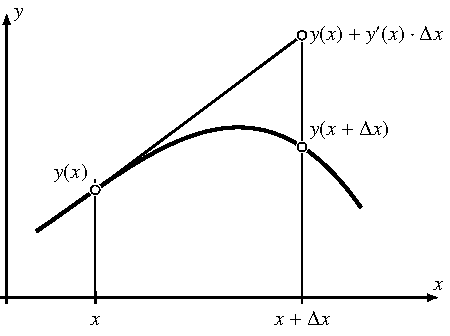
\includegraphics{chapters/50-ode/figures/prinzip.pdf}
\caption{Lineare Approximation von $y(x+\Delta x)$ durch Information,
die am Punkt $x$ verfügbar ist.
\label{buch:ode:lineareapproximation}}
\end{figure}
Wir versuchen als einführendes Beispiel, die Differentialgleichung
\begin{equation}
y'=-\alpha y,\qquad y(0)=y_0
\label{buch:ode:expdgl}
\end{equation}
numerisch zu lösen. 
Die Lösung ist natürlich bekannt, es ist 
\begin{equation}
y(x)=y_0e^{-\alpha x}.
\label{buch:ode:beispiel-loesung}
\end{equation}
Dazu unterteilen wir die $x$-Achse in diskrete Abschnitte der Länge $h$,
genannt die {\em Schrittweite},
\index{Schrittweite}%
und bezeichnen die Teilpunkte mit $x_k=kh$.
Das Ziel ist jetzt, $y(x_k)$ näherungsweise zu berechnen.
Wir schreiben $y_k$ für die Näherungswerte von $y(x_k)$.

Die Ableitung liefert eine lineare Approximation für $y(x)$,
\index{lineare Approximation}%
\index{Approximation!linear}%
nämlich
\[
y(x+\Delta x)\approx y(x) + y'(x)\cdot\Delta x
\]
(Abbildung~\ref{buch:ode:lineareapproximation}).
Für die Punkte $x_k$ bedeutet das
\[
y(x_{k+1})\approx y(x_{k})+y'(x_k)\cdot h.
\]
Die Differentialgleichung liefert Werte für $y'(x_k)$ aus $x_k$ und $y(x_k)$,
damit können wir aus dieser Approximation ein allgemeines
Näherungsverfahren für die Lösung einer Differentialgleichung
konstruieren.
\index{Näherungsverfahren}%

\begin{satz}[Euler-Verfahren]
\index{Euler-Verfahren}%
Die Differentialgleichung
\begin{equation}
y'=f(x,y),\qquad y(0)=y_0
\label{buch:ode:eulerdgl}
\end{equation}
und die Schrittweite $h$ definieren eine Folge 
\[
y_{\mathstrut k}=y_{k-1} + h\cdot f(x_{k-1}, y_{k-1}),\quad k>0,
\]
mit $x_k=kh$,
die eine Näherung für die Funktionswerte $y(x_k)$ der Lösung $y(x)$
der Differentialgleichung~\eqref{buch:ode:eulerdgl} ist.
\end{satz}

Dieses Verfahren ist nicht besonders gut, wie wir im Folgenden zeigen
wollen.
Die Diskussion soll vor allem zeigen, worauf bei der Weiterentwicklung
des Verfahrens geachtet werden muss.

Im vorliegenden Beispiel liefert die
Differentialgleichung~\eqref{buch:ode:expdgl}
den Wert $y'(x_k)=-\alpha y(x_k)$ für die Ableitung,
woraus wir die Rekursionsformel
\[
y_{k+1}=y_k - \alpha y_k \dot h.
\]
gewinnen.
Die Rekursionsgleichung kann in diesem Fall exakt gelöst werden,
und wir finden
\index{Rekursionsformel}%
\begin{equation}
y(x_{k+1}) = y(x_k)-\alpha y(x_k) h=(1-\alpha h) y(x_k)=\dots
=(1-\alpha h)^{k+1}y_0
\label{buch:ode:rekursion}
\end{equation}
für die Näherung $y_k$ der Funktionswerte $y(x_k)$.

Wir möchten $y(x)$ für einen ganz bestimmten $x$-Wert berechnen.
Dazu unterteilen wir das Intervall $[0,x]$ in $n$ Teilschritte der
Breite $x/n$, und wenden die Formel~\eqref{buch:ode:rekursion} an:
\[
y(x)=y(x_n)=(1-\alpha h)^n y_0=\biggl(1+\frac{-\alpha x}{n}\biggr)^n y_0.
\]
Für eine grosse Zahl von Teilschritten erhalten wir so tatsächlich die
korrekte Lösung:
\[
\lim_{n\to\infty}y_0\biggl(1+\frac{-\alpha x}n\biggr)^n=y_0 e^{-\alpha x}.
\]
\begin{figure}
\centering
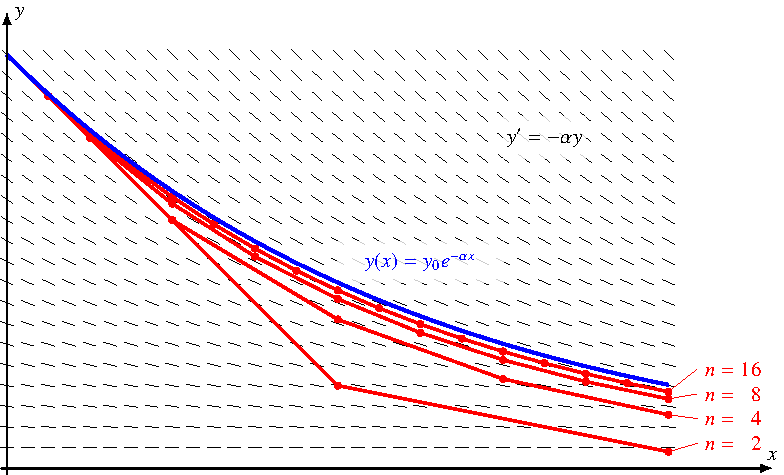
\includegraphics{chapters/50-ode/figures/euler.pdf}
\caption{Approximationen der Lösung der Differentialgleichung $y'=-\alpha y$
mit verschiedener Anzahl Schritte (rot) nähern sich für wachsendes
$n$ der exakten Lösung (blau).
\label{buch:ode:approximation}}
\end{figure}%
Abbildung~\ref{buch:ode:approximation} zeigt, wie die
durch~\eqref{buch:ode:rekursion} gegebenen Approximationen mit zunehmendem
$n$ der exakten Lösung $y(x)=e^{-\alpha x}$ näher kommen.

Wir können auch den Fehler des numerischen Verfahrens berechnen.
Bei der Schrittweite $h$ ist der Fehler von $y_k$ die Differenz
\[
y(x_k)-y_k
=
y_0e^{-\alpha kh}-y_0(1-\alpha h)^k
=
y_0((e^{-\alpha h})^k - (1-\alpha h)^k)
=
y_0e^{-\alpha hk}\biggl(
1-\biggl(\frac{1-\alpha h}{e^{-\alpha h}}\biggr)^k
\biggr).
\]
Man beachte, dass der Zähler $1-\alpha h$ die Approximation
$y_1$ ist, als eine Approximation von $e^{-\alpha h}$, dem Nenner.
Schreiben wir
\[
q=\frac{1-\alpha h}{e^{-\alpha h}},
\]
für den Quotienten zwischen der Approximation und dem korrekten Wert,
dann ist sicher immer $q<1$.
Den Fehler können wir jetzt schreiben
\[
y(x_k)-y_k = y_0e^{-\alpha hk}(1-q^k) = y(x_k)(1-q^k).
\]
Der relative Fehler des Verfahrens ist also
\[
\frac{y(x_k)-y_k}{y(x_k)}=(1-q^k).
\]
\begin{figure}
\centering
%\includegraphics{chapters/images/numerik-3.pdf}
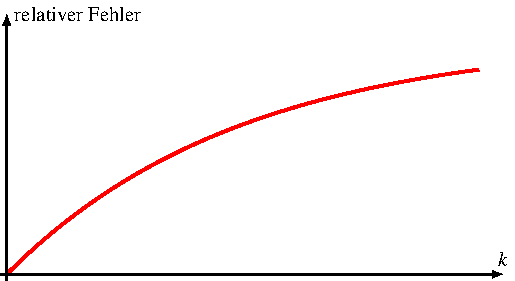
\includegraphics{chapters/50-ode/figures/relativ.pdf}
\caption{Relativer Fehler des Euler-Verfahrens für die Differentialgleichung
\eqref{buch:ode:expdgl} in Abhängigkeit von der Anzahl $k$ der Schritte.
\index{relativer Fehler}%
\label{buch:ode:relfehler}}
\end{figure}%
Ganz unabhängig von der Schrittweite $h$ wird der relative Fehler
des Verfahrens immer gegen 1 streben, der Fehler wird also von der
gleichen Grössenordnung wie die berechneten Resultate.
\index{Schrittweite}%

Die Abbildung~\ref{buch:ode:relfehler} zeigt, dass zu Beginn des Verfahrens
der relative Fehler ungefähr linear mit der Anzahl der Schritte zunimmt.
Um eine angemessene Genauigkeit über einen grösseren Bereich
zu erreichen, muss das Euler-Verfahren also sehr viel kleinere Schritte
und eine entsprechend grössere Anzahl von Schritten ausführen,
die viel Rechenzeit benötigen.
\index{Euler-Verfahren}%

Ein praktisch nützliches Verfahren muss also anstreben, mit einer
sehr viel kleineren Anzahl von Schritten eine deutlich grössere Genauigkeit
der Approximation zu erreichen.




\def\fehlerpfad#1#2{
\draw[line width=1.4pt,color=red] ({0.00000*#1},{0.00000*#2})
-- ({0.00500*#1},{0.00071*#2})
-- ({0.01000*#1},{0.00277*#2})
-- ({0.01500*#1},{0.00605*#2})
-- ({0.02000*#1},{0.01042*#2})
-- ({0.02500*#1},{0.01578*#2})
-- ({0.03000*#1},{0.02203*#2})
-- ({0.03500*#1},{0.02904*#2})
-- ({0.04000*#1},{0.03674*#2})
-- ({0.04500*#1},{0.04502*#2})
-- ({0.05000*#1},{0.05380*#2})
-- ({0.05500*#1},{0.06299*#2})
-- ({0.06000*#1},{0.07251*#2})
-- ({0.06500*#1},{0.08229*#2})
-- ({0.07000*#1},{0.09226*#2})
-- ({0.07500*#1},{0.10236*#2})
-- ({0.08000*#1},{0.11251*#2})
-- ({0.08500*#1},{0.12266*#2})
-- ({0.09000*#1},{0.13276*#2})
-- ({0.09500*#1},{0.14275*#2})
-- ({0.10000*#1},{0.15259*#2})
-- ({0.10500*#1},{0.16223*#2})
-- ({0.11000*#1},{0.17164*#2})
-- ({0.11500*#1},{0.18077*#2})
-- ({0.12000*#1},{0.18959*#2})
-- ({0.12500*#1},{0.19807*#2})
-- ({0.13000*#1},{0.20618*#2})
-- ({0.13500*#1},{0.21389*#2})
-- ({0.14000*#1},{0.22119*#2})
-- ({0.14500*#1},{0.22805*#2})
-- ({0.15000*#1},{0.23446*#2})
-- ({0.15500*#1},{0.24039*#2})
-- ({0.16000*#1},{0.24584*#2})
-- ({0.16500*#1},{0.25080*#2})
-- ({0.17000*#1},{0.25526*#2})
-- ({0.17500*#1},{0.25921*#2})
-- ({0.18000*#1},{0.26265*#2})
-- ({0.18500*#1},{0.26557*#2})
-- ({0.19000*#1},{0.26798*#2})
-- ({0.19500*#1},{0.26987*#2})
-- ({0.20000*#1},{0.27126*#2})
-- ({0.20500*#1},{0.27213*#2})
-- ({0.21000*#1},{0.27251*#2})
-- ({0.21500*#1},{0.27240*#2})
-- ({0.22000*#1},{0.27180*#2})
-- ({0.22500*#1},{0.27073*#2})
-- ({0.23000*#1},{0.26919*#2})
-- ({0.23500*#1},{0.26721*#2})
-- ({0.24000*#1},{0.26479*#2})
-- ({0.24500*#1},{0.26194*#2})
-- ({0.25000*#1},{0.25869*#2})
-- ({0.25500*#1},{0.25505*#2})
-- ({0.26000*#1},{0.25104*#2})
-- ({0.26500*#1},{0.24666*#2})
-- ({0.27000*#1},{0.24195*#2})
-- ({0.27500*#1},{0.23693*#2})
-- ({0.28000*#1},{0.23160*#2})
-- ({0.28500*#1},{0.22599*#2})
-- ({0.29000*#1},{0.22012*#2})
-- ({0.29500*#1},{0.21401*#2})
-- ({0.30000*#1},{0.20769*#2})
-- ({0.30500*#1},{0.20116*#2})
-- ({0.31000*#1},{0.19447*#2})
-- ({0.31500*#1},{0.18761*#2})
-- ({0.32000*#1},{0.18063*#2})
-- ({0.32500*#1},{0.17353*#2})
-- ({0.33000*#1},{0.16634*#2})
-- ({0.33500*#1},{0.15908*#2})
-- ({0.34000*#1},{0.15178*#2})
-- ({0.34500*#1},{0.14445*#2})
-- ({0.35000*#1},{0.13711*#2})
-- ({0.35500*#1},{0.12979*#2})
-- ({0.36000*#1},{0.12250*#2})
-- ({0.36500*#1},{0.11527*#2})
-- ({0.37000*#1},{0.10812*#2})
-- ({0.37500*#1},{0.10106*#2})
-- ({0.38000*#1},{0.09411*#2})
-- ({0.38500*#1},{0.08730*#2})
-- ({0.39000*#1},{0.08063*#2})
-- ({0.39500*#1},{0.07414*#2})
-- ({0.40000*#1},{0.06782*#2})
-- ({0.40500*#1},{0.06171*#2})
-- ({0.41000*#1},{0.05581*#2})
-- ({0.41500*#1},{0.05014*#2})
-- ({0.42000*#1},{0.04472*#2})
-- ({0.42500*#1},{0.03955*#2})
-- ({0.43000*#1},{0.03466*#2})
-- ({0.43500*#1},{0.03005*#2})
-- ({0.44000*#1},{0.02574*#2})
-- ({0.44500*#1},{0.02173*#2})
-- ({0.45000*#1},{0.01803*#2})
-- ({0.45500*#1},{0.01466*#2})
-- ({0.46000*#1},{0.01162*#2})
-- ({0.46500*#1},{0.00893*#2})
-- ({0.47000*#1},{0.00658*#2})
-- ({0.47500*#1},{0.00458*#2})
-- ({0.48000*#1},{0.00293*#2})
-- ({0.48500*#1},{0.00165*#2})
-- ({0.49000*#1},{0.00074*#2})
-- ({0.49500*#1},{0.00018*#2})
-- ({0.50000*#1},{0.00000*#2})
-- ({0.50500*#1},{0.00018*#2})
-- ({0.51000*#1},{0.00074*#2})
-- ({0.51500*#1},{0.00165*#2})
-- ({0.52000*#1},{0.00293*#2})
-- ({0.52500*#1},{0.00458*#2})
-- ({0.53000*#1},{0.00658*#2})
-- ({0.53500*#1},{0.00893*#2})
-- ({0.54000*#1},{0.01162*#2})
-- ({0.54500*#1},{0.01466*#2})
-- ({0.55000*#1},{0.01803*#2})
-- ({0.55500*#1},{0.02173*#2})
-- ({0.56000*#1},{0.02574*#2})
-- ({0.56500*#1},{0.03005*#2})
-- ({0.57000*#1},{0.03466*#2})
-- ({0.57500*#1},{0.03955*#2})
-- ({0.58000*#1},{0.04472*#2})
-- ({0.58500*#1},{0.05014*#2})
-- ({0.59000*#1},{0.05581*#2})
-- ({0.59500*#1},{0.06171*#2})
-- ({0.60000*#1},{0.06782*#2})
-- ({0.60500*#1},{0.07414*#2})
-- ({0.61000*#1},{0.08063*#2})
-- ({0.61500*#1},{0.08730*#2})
-- ({0.62000*#1},{0.09411*#2})
-- ({0.62500*#1},{0.10106*#2})
-- ({0.63000*#1},{0.10812*#2})
-- ({0.63500*#1},{0.11527*#2})
-- ({0.64000*#1},{0.12250*#2})
-- ({0.64500*#1},{0.12979*#2})
-- ({0.65000*#1},{0.13711*#2})
-- ({0.65500*#1},{0.14445*#2})
-- ({0.66000*#1},{0.15178*#2})
-- ({0.66500*#1},{0.15908*#2})
-- ({0.67000*#1},{0.16634*#2})
-- ({0.67500*#1},{0.17353*#2})
-- ({0.68000*#1},{0.18063*#2})
-- ({0.68500*#1},{0.18761*#2})
-- ({0.69000*#1},{0.19447*#2})
-- ({0.69500*#1},{0.20116*#2})
-- ({0.70000*#1},{0.20769*#2})
-- ({0.70500*#1},{0.21401*#2})
-- ({0.71000*#1},{0.22012*#2})
-- ({0.71500*#1},{0.22599*#2})
-- ({0.72000*#1},{0.23160*#2})
-- ({0.72500*#1},{0.23693*#2})
-- ({0.73000*#1},{0.24195*#2})
-- ({0.73500*#1},{0.24666*#2})
-- ({0.74000*#1},{0.25104*#2})
-- ({0.74500*#1},{0.25505*#2})
-- ({0.75000*#1},{0.25869*#2})
-- ({0.75500*#1},{0.26194*#2})
-- ({0.76000*#1},{0.26479*#2})
-- ({0.76500*#1},{0.26721*#2})
-- ({0.77000*#1},{0.26919*#2})
-- ({0.77500*#1},{0.27073*#2})
-- ({0.78000*#1},{0.27180*#2})
-- ({0.78500*#1},{0.27240*#2})
-- ({0.79000*#1},{0.27251*#2})
-- ({0.79500*#1},{0.27213*#2})
-- ({0.80000*#1},{0.27126*#2})
-- ({0.80500*#1},{0.26987*#2})
-- ({0.81000*#1},{0.26798*#2})
-- ({0.81500*#1},{0.26557*#2})
-- ({0.82000*#1},{0.26265*#2})
-- ({0.82500*#1},{0.25921*#2})
-- ({0.83000*#1},{0.25526*#2})
-- ({0.83500*#1},{0.25080*#2})
-- ({0.84000*#1},{0.24584*#2})
-- ({0.84500*#1},{0.24039*#2})
-- ({0.85000*#1},{0.23446*#2})
-- ({0.85500*#1},{0.22805*#2})
-- ({0.86000*#1},{0.22119*#2})
-- ({0.86500*#1},{0.21389*#2})
-- ({0.87000*#1},{0.20618*#2})
-- ({0.87500*#1},{0.19807*#2})
-- ({0.88000*#1},{0.18959*#2})
-- ({0.88500*#1},{0.18077*#2})
-- ({0.89000*#1},{0.17164*#2})
-- ({0.89500*#1},{0.16223*#2})
-- ({0.90000*#1},{0.15259*#2})
-- ({0.90500*#1},{0.14275*#2})
-- ({0.91000*#1},{0.13276*#2})
-- ({0.91500*#1},{0.12266*#2})
-- ({0.92000*#1},{0.11251*#2})
-- ({0.92500*#1},{0.10236*#2})
-- ({0.93000*#1},{0.09226*#2})
-- ({0.93500*#1},{0.08229*#2})
-- ({0.94000*#1},{0.07251*#2})
-- ({0.94500*#1},{0.06299*#2})
-- ({0.95000*#1},{0.05380*#2})
-- ({0.95500*#1},{0.04502*#2})
-- ({0.96000*#1},{0.03674*#2})
-- ({0.96500*#1},{0.02904*#2})
-- ({0.97000*#1},{0.02203*#2})
-- ({0.97500*#1},{0.01578*#2})
-- ({0.98000*#1},{0.01042*#2})
-- ({0.98500*#1},{0.00605*#2})
-- ({0.99000*#1},{0.00277*#2})
-- ({0.99500*#1},{0.00071*#2})
-- ({1.00000*#1},{0.00000*#2});
}

%
% einschritt.tex -- 
%
% (c) 2015 Prof Dr Andreas Mueller, Hochschule Rapperswil
%
\section{Einschrittverfahren\label{buch:section:ode:einschritt}}
\rhead{Einschrittverfahren}
\index{Einschrittverfahren}%
Die relativ geringe Genauigkeit des Euler-Schrittes beruht darauf,
dass die zu Beginn des Schrittes berechnete Ableitung $f(x_k,y_k)$
nur für das linke Ende des Intervalls $[x_k, x_k+h]$ zutrifft,
weiter rechts im Intervall wird die Abweichung immer grösser.
Eine mögliche Lösung des Problems könnte darin bestehen, statt
nur einer linearen Näherung zusätzliche Glieder der Taylor-Reihe
\begin{equation}
y(x+\Delta x)
=
y(x)
+
y'(x)\cdot \Delta x
+
\frac12 y''(x)\cdot \Delta x^2
+
\frac16 y'''(x)\cdot \Delta x^3
+
o(\Delta x^3)
\label{buch:ode:taylor}
\end{equation}
zu verwenden.
In \eqref{buch:ode:taylor} werden höhere Ableitungen von $y(x)$ benötigt,
während die Differentialgleichung nur die erste Ableitung liefert.
Die höheren Ableitungen wurden aber bereits im
Abschnitt~\ref{grundlagen:hoehere-ableitungen} berechnet.

Wir untersuchen, wie sich das Verfahren für die Beispiel-Gleichung
\eqref{buch:ode:expdgl} anwenden lässt.
Dort gilt
\begin{equation*}
\begin{aligned}
y'(x)&=f(x,y)=-\alpha y
\\
\Rightarrow\qquad
\frac{\partial f}{\partial x}&=0&\frac{\partial f}{\partial y}&=-\alpha.
\end{aligned}
\end{equation*}
Alle zweiten Ableitungen verschwinden.
Die Gleichungen werden damit einfach:
\begin{align*}
y''(x)&=-\alpha f(x,y)=\alpha^2 y
\\
y'''(x)&=\alpha^2f(x,y)=-\alpha^3 y.
\end{align*}
Statt der linearen Approximation sollte daher die kubische Approximation
\begin{equation}
y_{k+1}
=
y_{k}-\alpha h y_k +\frac12\alpha^2 h^2 y_k -\frac16 \alpha^3h^3 y_k
=
y_{k}\underbrace{\biggl(1-\alpha h +\frac12\alpha^2h^2 -\frac16 \alpha^3h^3\biggr)}_{\displaystyle \approx e^{-\alpha h}}
\label{buch:ode:kubisch}
\end{equation}
verwendet werden.
Dass man hier mit einer grösseren Genauigkeit rechnen darf, ist schon daran
erkennbar, dass der Klammerausdruck auf der rechten Seite eine viel
bessere Approximation von $e^{-\alpha x}$ ist also der Faktor
$(1-\alpha h)$ im Euler-Verfahren.
Genauer erwarten wir, dass wir hier ein kubisches Verfahren konstruiert haben.

\begin{table}
\centering
\begin{tabular}{|r|c|r|r|r|}
\hline
$i$&$x$&$e^{-\alpha x}$&Euler&kubisch\\
\hline
 1 & 0.1 & 0.95122942 & 0.\underline{95}000000 & 0.\underline{951229}17 \\
 2 & 0.2 & 0.90483742 & 0.\underline{90}250000 & 0.\underline{904836}93 \\
 3 & 0.3 & 0.86070798 & 0.\underline{85}737500 & 0.\underline{860707}28 \\
 4 & 0.4 & 0.81873075 & 0.\underline{81}450625 & 0.\underline{818729}87 \\
 5 & 0.5 & 0.77880078 & 0.\underline{77}378094 & 0.\underline{778799}73 \\
 6 & 0.6 & 0.74081822 & 0.\underline{73}509189 & 0.\underline{74081}702 \\
 7 & 0.7 & 0.70468809 & 0.\underline{6}9833730 & 0.\underline{70468}675 \\
 8 & 0.8 & 0.67032005 & 0.\underline{6}6342043 & 0.\underline{67031}859 \\
 9 & 0.9 & 0.63762815 & 0.\underline{6}3024941 & 0.\underline{63762}660 \\
10 & 1.0 & 0.60653066 & 0.\underline{5}9873694 & 0.\underline{60652}902 \\
\hline
\end{tabular}
\caption{Näherungswerte für die Lösung $e^{-\alpha x}$ der
Beispieldifferentialgleichung \eqref{buch:ode:expdgl} nach dem Euler-Verfahren
und nach dem kubischen Verfahren \eqref{buch:ode:kubisch} mit einer
Schrittweite von 0.1. Unterstrichen ist jeweils die Stellen, die nach
Rundung auf die angegebene Anzahl stellen mit dem exakten Wert übereinstimmt.
\label{buch:ode:euler-kubisch}}
\end{table}%
In Tabelle~\ref{buch:ode:euler-kubisch} werden die Resultate des
kubischen Verfahrens denen des Euler-Verfahrens gegenübergestellt.
Im ersten Schritt ist der Fehler des Euler-Verfahrens kleiner als $10^{-2}$,
was einer Einheit in der zweiten Nachkommastelle entspricht.
Der Fehler des kubischen Verfahrens ist kleiner als $10^{-6}$, eine
Einheit in der sechsten Nachkommastelle, ungefähr die von einem
kubischen Verfahren zu erwartende Verbesserung.
Nach zehn Rechenschritten liefert das Euler-Verfahren dank Rundung
gerade noch eine korrekte Stelle, während das kubische Verfahren immer noch
gerundet fünf korrekte Stellen gibt.

Es wurde bereits darauf hingewiesen, dass die Terme für die Ableitungen
sehr kompliziert werden.
Noch viel gravierender ist allerdings, dass auch die partiellen Ableitungen
von $f$ nach $x$ und $y$ bekannt sein müssen.
Es ist zwar im Prinzip möglich, diese zu berechnen, der Rechenaufwand 
dafür kann aber so erheblich sein, dass er den Genauigkeitsgewinn
leicht wieder zunichte machen kann.
Praktisch nützliche Verfahren müssen daher danach streben,
die höheren Ableitungen von $y(x)$ ausschliesslich aus Funktionswerten
von $f(x,y)$ zu berechnen.

Wir möchten aber weiterhin nur $y_{k+1}$ ausschliesslich aus $x_k$ und $y_k$
berechnen, also in einem einzelnen Schritt der Form
\[
y_{k+1}=y_k + h\, F(x_k, y_k, h).
\]
Die Funktion $F(x,y,h)$ heisst die {\em Inkrementfunktion}
\index{Inkrementfunktion}%
des Verfahrens.
Für das Euler-Verfahren ist $F(x,y,h)=f(x,y)$.
Es soll also eine Inkrementfunktion gefunden werden, bei der $y(x+\Delta x)$
durch $y(x) + \Delta x\cdot F(x,y,\Delta x)$ bis auf Terme höherer
Ordnung approximiert werden kann.

\subsection{Quadratische Verfahren\label{buch:subsection:quadratischeverfahren}}
\index{quadratische!Verfahren}%
Ein quadratisches Verfahren verwendet eine Inkrementfunktion $F(x,y,h)$,
welche
\[
y(x+h)=y(x)+hF(x,y,h)+O(h^3)
\]
erfüllt.
Aus den einleitenden Bemerkungen von~\ref{buch:section:ode:einschritt}
folgt, dass dieses Ziel möglicherweise dadurch erreicht werden kann,
dass man Werte von $f$ für verschiedene $x$ geeignet miteinander
kombiniert.
Ein denkbarer Ansatz dafür ist
\[
F(x,y,h)=af(x,y) + bf(x+\alpha h, y +\beta hf(x,y)),
\]
oder anders ausgedrückt: Man führt zuerst etwas Ähnliches wie einen
Euler-Schritt durch, um zum Punkt $(x+\alpha h,y+\beta hf(x,y))$ zu
gelangen.
\index{Euler-Schritt}%
Dort berechnet man den Wert von $f$ und bildet dann einen geeigneten
Mittelwert davon  mit $f(x,y)$.
Durch geeignete Wahl von $a$, $b$, $\alpha$ und $\beta$ sollte es möglich
sein, dass die Inkrementfunktion einen Fehler höchstens dritter Ordnung
hat, womit wir dann ein Integrationsverfahren zweiter Ordnung gewonnen
hätten.

Wir müssen jetzt die Parameter $a$, $b$, $\alpha$ und $\beta$ bestimmen.
Da wir mit dem Übereinstimmen der ersten zwei Ableitungen
nur zwei Bedingungen haben, können wir nicht erwarten, dass wir
eine eindeutige Lösung finden werden.
Vielmehr werden einzelne Parameter frei wählbar sein, es wird eine
ganze Familie von quadratischen Lösungsverfahren entstehen, parametrisiert
durch eine der Variablen $a$, $b$, $\alpha$ und $\beta$.

Wir berechnen nun $F(x,y,h)$ bis zur zweiten Ordnung, damit wird 
$y(x+h)$ bis zur dritten Ordnung ausdrücken können:
\begin{align}
f(x+\alpha h, y + \beta h f(x,y))
&=
f(x,y)+\alpha h\frac{\partial f(x,y)}{\partial x}
+ \beta h \frac{\partial f(x,y)}{\partial y} + O(h^2)
\notag
\\
F(x,y,h)
&=
af(x,y) + bf(x+\alpha h, y + \beta h f(x,y))
\notag
\\
&=
(a+b)f(x,y) + \biggl(\alpha b\frac{\partial f(x,y)}{\partial x}
+ \beta b\frac{\partial f(x,y)}{\partial y} f(x,y))\biggr)h+O(h^2).
\label{buch:ode:inkrementF}
\end{align}
Damit dies bis zur zweiten Ordnung mit dem Inkrement zwischen $x$ und $x+h$
übereinstimmt, muss~\eqref{buch:ode:inkrementF} mit der Taylor-Reihe
von $y(x)$ übereinstimmen, also mit
\begin{equation}
\frac{y(x+h)-y(x)}{h}=y'(x) + \frac12y''(x)h + O(h^2)
=f(x,y) + \frac12\frac{\partial f(x,y)}{\partial x}
+\frac12\frac{\partial f(x,y)}{\partial y}f(x,y) + O(h^2),
\label{buch:ode:ytaylor}
\end{equation}
wobei wir für $y''(x)$ die Gleichung \eqref{grundlagen:2abl} verwendet haben.
Durch Koeffizientenvergleich finden wir die Bedingungen
\[
\begin{aligned}
a+b&=1,&
\alpha b&=\frac12,&
\beta b&=\frac12.
\end{aligned}
\]
Einzig $b$ kommt in allen drei Gleichungen vor und bestimmt den Wert der
jeweiligen anderen Variablen:
\[
\begin{aligned}
a&=1-b,&\alpha&= \beta=\frac{1}{2b}.
\end{aligned}
\]
Jeder Wert von $b$ zwischen $0$ und $1$ liefert ein Verfahren mit quadratischer
Genauigkeit.

\begin{figure}
\centering
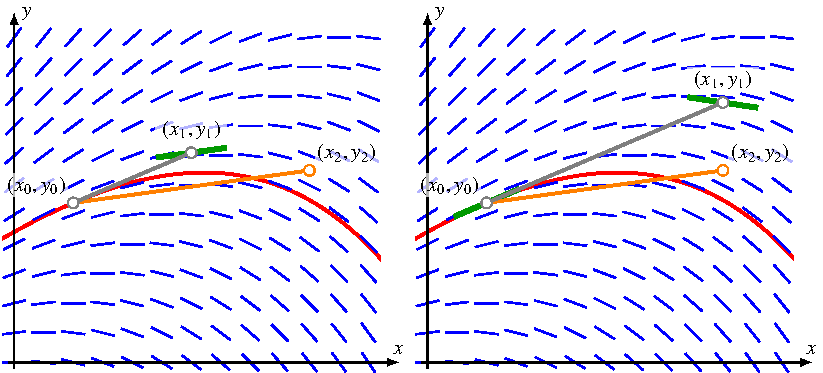
\includegraphics{chapters/50-ode/figures/ordnung2.pdf}
\caption{Einschrittverfahren zweiter Ordnung.
\index{Euler-Verfahren!verbessert}%
\index{verbessertes Euler-Verfahren}%
Das verbesserte Euler-Verfahren (links) führt zunächst einen Euler-Schritt
halber Länge mit der Steigung $f(x_0,y_0)$ (grau) aus und verwendet
die bei $(x_1,y_1)$ gefundene Steigung 
$f(x_1,y_1)$ (grün) für einen ganzen Euler-Schritt (orange),
der zu $(x_2,y_2)$ führt.
\index{Runge-Kutta-Verfahren!vereinfacht}%
\index{vereinfachtes Runge-Kutta-Verfahren}%
Das vereinfachte Runge-Kutta-Verfahren (rechts) führt einen ganzen
Euler-Schritt (grau) aus, der zu $(x_1,y_1)$ führt.
Dann wird der Mittelwert der Steigungen $f(x_0,y_0)$ und $f(x_1,y_1)$
(grün) für einen ganzen Euler-Schritt verwendet, der zu $(x_2,y_2)$ führt
(orange).
\label{buch:einschritt:figure:ordnung2}}
\end{figure}

Der Parameterwert $b=1$ führt auf $\alpha=\beta=1$ und $a=0$, die
Rekursionsformel ist in diesem Falle
\begin{equation}
y_{k+1}=y_{k}+hf\biggl(x_k+\frac{h}2,y_k+\frac{h}2 f(x_k,y_k)\biggr).
\label{buch:ode:improved-euler}
\end{equation}
Das Verfahren führt also erst einen halben Euler-Schritt zum Punkt
$(x_k+\frac12h,y_k+\frac{h}2f(x_k,y_k))$ durch, berechnet dort mit Hilfe
von $f$ die Steigung, die dann für einen Euler-Schritt der Länge $h$
verwendet wird
(Abbildung~\ref{buch:einschritt:figure:ordnung2} links).
Daher heisst dieses Verfahren auch das {\em verbesserte Euler-Verfahren}.
\index{Euler-Verfahren!verbessert}%
\index{verbessertes Euler-Verfahren}%

Verwendet man $b=\frac12$, folgt zunächst $a=\frac12$ und $\alpha=\beta=1$.
Daraus erhält man die Rekursionsformel
\begin{equation}
y_{k+1}=y_k+\frac{h}2\biggl(
f(x_k,y_k) + f(x_k+h, y_k + hf(x_k,y_k))
\biggr).
\label{buch:ode:simplified-runge-kutta}
\end{equation}
In diesem Verfahren
(Abbildung~\ref{buch:einschritt:figure:ordnung2} rechts)
führt man also zuerst einen Euler-Schritt der Länge
$h$ durch, mit dem man zum Punkt $(x_k+h, y_k+hf(x_k,y_k))$ gelangt.
Dort berechnet mit mit Hilfe von $f$ die Steigung.
Das arithmetische Mittel dieser Steigung mit der im Euler-Verfahren
verwendeten Steigung $f(x_k,y_k)$ im Punkt $x_k$ wird dann als
Steigung für einen Euler-Schritt verwendet.
Statt eines einzigen Steigungswertes werden hier also zwei Steigungswerte
von den Enden des Intervalls $[x_k,x_{k+1}]$ gemittelt.
Wegen der Ähnlichkeit dieses Vorgehens mit dem später zu besprechenden
Runge-Kutte-Verfahren heisst diese Verfahren auch das
{\em vereinfachte Runge-Kutta-Verfahren}.
\index{Runge-Kutta-Verfahren!vereinfacht}%
\index{vereinfachtes Runge-Kutta-Verfahren}%

\subsection{Runge-Kutta-Verfahren\label{subsection:buch:ode:runge-kutta}}
\index{Runge-Kutta-Verfahren}%
\begin{figure}
\centering
%\includegraphics{chapters/images/numerik-4.pdf}
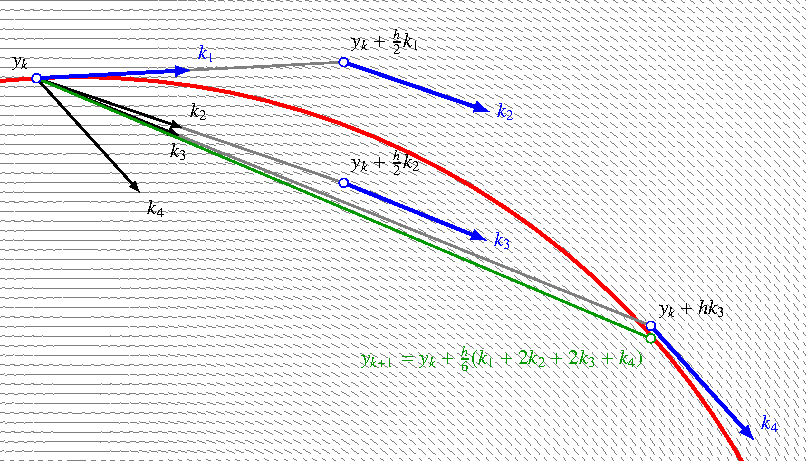
\includegraphics{chapters/50-ode/figures/rungekutta.pdf}
\caption{Zusammenspiel der Richtungen $k_1$ bis $k_4$ bei einem
Einzelschritt des Runge-Kutta-Verfahrens vierter Ordnung.
Der nächste Punkt $y_{k+1}$ wird gemäss
Formel~\eqref{buch:ode:runge-kutta-rekursion} berechnet.
\index{Runge-Kutta-Verfahren}%
\label{buch:ode:rk-step}}
\end{figure}
Das {\em Runge-Kutta-Verfahren} erweitert die Inkrementfunktion derart,
dass der Einzelschritt bis zur fünften Ordnung mit der Taylor-Reihe von
$y(x)$ übereinstimmt.
\index{Taylor-Reihe}%
\index{Runge-Kutta-Verfahren}%
So entsteht ein Verfahren vierter Ordnung, es stellt einen guten Kompromiss
zwischen Genauigkeit und Rechenaufwand dar.
\index{Genauigkeit}%
\index{Rechenaufwand}%

Da vier Ableitungen korrekt dargestellt werden müssen, ist zu erwarten,
dass vier verschiedene Werte von $f$ an verschiedenen Punkten $(x,y)$
ausgewertet und geeignet miteinander kombiniert werden müssen.
Genauer: Man bestimmt zuerst die Werte
\begin{align*}
k_1&=f(x_k,y_k)\\
k_2&=f\biggl(x_k+\frac{h}2,y_k+\frac{h}2k_1\biggr)\\
k_3&=f\biggl(x_k+\frac{h}2,y_k+\frac{h}2k_2\biggr)\\
k_4&=f(x_k+h, y_k+hk_3)
\end{align*}
und setzt diese dann zusammen, um den nächsten Wert $y_{k+1}$
zu berechnen:
\begin{equation}
y_{k+1} = y_k + \frac{h}6(k_1 + 2k_2 + 2k_3 + k_4)
\label{buch:ode:runge-kutta-rekursion}
\end{equation}
(Abbildung~\ref{buch:ode:rk-step}).
Man kann die Formeln wie folgt interpretieren.
\begin{enumerate}
\item
Zuerst wird ein halber Euler-Schritt mit der Steigung $k_1=f(x_k,y_k)$
durchgeführt und am Zielpunkt die Steigung $k_2$ ermittelt.
\item
Mit dieser Steigung $k_2$ wird dann erneut ein halber Schritt von $(x_k,y_k)$
aus durchgeführt und am Zielpunkt erneut die Steigung $k_3$ ermittelt.
\item
Mit $k_3$ führt man einen ganzen Schritt aus, an dessen Zielpunkt man die
Steigung $k_4$ findet.
\item
Diese vier Steigungen werden jetzt gewichtet gemittelt, wobei
$k_2$ und $k_3$ doppeltes Gewicht erhalten, und mit dieser
Steigung wird ein ganzer Schritt vorgenommen.
\end{enumerate}

Die Formeln für die $k_i$ sowie \eqref{buch:ode:runge-kutta-rekursion}
können ganz ähnlich wie das verbesserte Euler-Verfahren bzw.~das
vereinfachte Runge-Kutta-Verfahren begründet werden.
Der Aufwand dafür ist aber beträchtlich, so dass wir auf die
detaillierte Darstellung dieser Herleitung verzichten wollen.

\begin{table}
\centering
\begin{tabular}{|r|c|r|r|r|r|r|}
\hline
$i$& $x$ & $y(x)=e^{-\alpha x}$&Euler&verbessert&vereinfacht&Runge-Kutta\\
\hline
 0 & 0.0 & 1.00000000 & 1.000 & 1.00000000 & 1.00000000 & 1.0000000000 \\
 1 & 0.1 & 0.95122942 & 0.\underline{95}0 & 0.\underline{9512}5000 & 0.\underline{9512}5000 & 0.\underline{95122942}71 \\
 2 & 0.2 & 0.90483742 & 0.\underline{90}2 & 0.\underline{9048}7656 & 0.\underline{9048}7656 & 0.\underline{9048374}229 \\
 3 & 0.3 & 0.86070798 & 0.\underline{85}7 & 0.\underline{8607}6383 & 0.\underline{8607}6383 & 0.\underline{8607079}834 \\
 4 & 0.4 & 0.81873075 & 0.\underline{81}4 & 0.\underline{8188}0159 & 0.\underline{8188}0159 & 0.\underline{8187307}620 \\
 5 & 0.5 & 0.77880078 & 0.\underline{77}3 & 0.\underline{7788}8502 & 0.\underline{7788}8502 & 0.\underline{7788007}936 \\
 6 & 0.6 & 0.74081822 & 0.\underline{73}5 & 0.\underline{7409}1437 & 0.\underline{7409}1437 & 0.\underline{7408182}327 \\
 7 & 0.7 & 0.70468809 & 0.\underline{69}8 & 0.\underline{704}79480 & 0.\underline{704}79480 & 0.\underline{7046881}031 \\
 8 & 0.8 & 0.67032005 & 0.\underline{6}63 & 0.\underline{670}43605 & 0.\underline{670}43605 & 0.\underline{6703200}606 \\
 9 & 0.9 & 0.63762815 & 0.\underline{6}30 & 0.\underline{637}75229 & 0.\underline{637}75229 & 0.\underline{6376281}672 \\
10 & 1.0 & 0.60653066 & 0.\underline{5}98 & 0.\underline{606}66187 & 0.\underline{606}66187 & 0.\underline{6065306}762 \\
\hline
\end{tabular}
\caption{Vergleich der Genauigkeit der verbesserten numerischen Verfahren.
Unterstrichen jeweils die nach Rundung korrekten Stellen der Lösung.
\label{buch:ode:genauigkeit}}
\end{table}


\begin{table}
\centering
\begin{tabular}{|l|l|c|r|>{$}r<{$}|}
\hline
Verfahren                           &$h$  &Schritte&$y_n$&\text{Fehler}\\
\hline
Euler-Verfahren                     &0.025&  40    & 0.\underline{60}462232 &  0.00190834 \\
verbessertes Euler-Verfahren        &0.05 &  20    & 0.\underline{6065}6285 & -0.00003219 \\
vereinfachtes Runge-Kutta-Verfahren &0.05 &  20    & 0.\underline{6065}6285 & -0.00003219 \\
Runge-Kutta-Verfahren               &0.1  &  10    & 0.\underline{6065306}7 & -0.00000001 \\
\hline
\end{tabular}
\caption{Vergleich der verschiedenen Verfahren bei gleichbleibendem 
Rechenaufwand.
\index{Schrittweite}%
Die Schrittweite wurde jeweils so angepasst, dass in allen Verfahren bis
zum Wert $x=1$ die gleiche Anzahl von Auswertungen der Funktion $f$
notwendig wurde.
\label{buch:ode:vergleich-aufwand}}
\end{table}

Die Tabelle~\ref{buch:ode:genauigkeit} demonstriert die überragende
Genauigkeit des Runge-Kutta-Verfahrens.
\index{Genauigkeit}%
Trotz der relativ grossen Schrittweite von $h=0.1$ erreicht das
Verfahren nach zehn Schritten eine Genauigkeit von sieben signifikanten
Stellen.
Da in jedem Schritt die Funktion $f$ viermal ausgewertet werden muss,
ist der Rechenaufwand mit dem Runge-Kutta-Verfahren viermal grösser
als im Euler-Verfahren, letzteres kann aber mit nur einer signifikanten
Stelle kaum als brauchbar bezeichnet werden.
\index{Euler-Verfahren}%
Passt man in jedem Verfahren die Schrittweite so an, dass für die
Berechnung der Näherung für $y(1)$ immer gleich viele Auswertungen
der Funktion $f(x,y)$ nötig sind, ergeben sich die Resultate in
Tabelle~\ref{buch:ode:vergleich-aufwand}.
Bei gleichem Rechenaufwand ist das Runge-Kutta-Verfahren um viele
Grössenordnungen präziser.
Es gibt daher eigentlich keinen praktischen Grund, überhaupt je etwas
anderes als das Runge-Kutta-Verfahren zu verwenden.



%
% mehrschritt.tex
%
% (c) 2020 Prof Dr Andreas Müller, Hochschule Rapperswil
%
\begin{frame}
\frametitle{Mehrschrittverfahren}
\begin{block}{Einschritt-Verfahren}
\vspace{-5pt}
\[
\hspace{-8pt}
y_{k+1}
=
y_k + hF(x_k,y_k,h)
\hspace*{7.7cm}
\]
\end{block}
\uncover<2->{%
\begin{block}{Mehrschritt-Verfahren}
\vspace{-15pt}
\begin{align*}
y_{k+1}
&\uncover<3->{=
y_k + h f(x_k,y_k)}
&&\uncover<7->{O(h)}
\\
&\uncover<4->{=
y_k + h
\biggl(
\frac{3}{2} f(x_k,y_k) + \frac12 f(x_{k-1},y_{k-1})
\biggr)}
&&\uncover<7->{O(h^2)}
\\
&\uncover<5->{=
y_k + h
\biggl(
\frac{23}{12} f(x_k,y_k) -\frac{4}{3}f(x_{k-1},y_{k-1}) + \frac{5}{12}f(x_{k-2},y_{k-2})
\biggr)}
&&\uncover<7->{O(h^3)}
\\
&\uncover<6->{=
y_k + h
\biggl(
\frac{55}{24} f(x_k,y_k) -\frac{59}{24}f(x_{k-1},y_{k-1})\\
&\qquad  + \frac{37}{24}f(x_{k-2},y_{k-2}) -\frac{3}{8}f(x_{k-3},y_{k-3})
\biggr)}
&&\uncover<7->{O(h^4)}
\end{align*}
\end{block}}
\end{frame}

%
% software.tex -- 
%
% (c) 2015 Prof Dr Andreas Mueller, Hochschule Rapperswil
%
\section{Software}
\rhead{Software}
Die im letzten Abschnitt entwickelten numerischen Verfahren zur Lösung
einer Differentialgleichung kommen ausschliesslich mit Auswertungen der
Funktion $f$ aus, die Ableitungen der Funktion $f$ müssen nicht bekannt
sein.
Es sollte also ein Leichtes sein, eine Softwarebibliothek zur
Verfügung zu stellen, mit der eine beliebige gewöhnliche
Differentialgleichung gelöst werden kann.
Als Input braucht es nur die Funktion $f$ und die Anfangsbedingungen.

Als Beispiel wollen wir in diesem Abschnitt die Differentialgleichung
\[
y''+y=\sin \frac{x}{10},\qquad y(0)=y'(0)=0
\]
in verschiedenen Programmierumgebungen lösen.
Als erstes bringen wir die Differentialgleichung wieder in die Standardform
einer Vektordifferentialgleichung erste Ordnung:
\begin{equation}
\frac{d}{dt}Y
=
\frac{d}{dx}\begin{pmatrix}y_1\\y_2\end{pmatrix}
=
\begin{pmatrix}
y_2\\
\displaystyle -y_1+\sin\frac{x}{10}
\end{pmatrix}
=
f(x,Y).
\label{buch:ode:beispieldgl}
\end{equation}
Ein numerisches Verfahren braucht also als Input eine Anfangsbedingung
sowie die Funktion $f$.
Ausserdem muss es Möglichkeiten bereitstellen, wie man den Gang der
Rechnung beeinflussen kann, z.~B.~um die $x$-Werte anzugeben, für die
die $Y(x)$ bestimmt werden sollen, oder um Genauigkeitsziele zu erreichen.

\subsection{Octave}
\index{Octave}%
In Octave steht eine einzige Funktion \texttt{lsode} zur Verfügung, welche
\index{lsode@{\texttt{lsode}}}
auf zuverlässige Art Differentialgleichungen löst.
Der Anwender muss eine Implementation der Funktion $f$ zur Verfügung
stellen, allerdings werden die Argument in der umgekehrten Reihenfolge
zu der erwarte, die wir in diesem Skript bisher verwendet haben.
Für die Beispieldifferentialgleichung \eqref{buch:ode:beispieldgl}
kann man sie zum Beispiel so definieren:
\lstinputlisting[style=Octave]{chapters/50-ode/examples/octave-dgl-f.m}

Beim Aufruf der Funktion \texttt{lsode} muss man den {\em Namen}
der Funktion, die Anfangsbedingung, sowie einen Vektoren mit $x$-Werten,
für die man die Lösung ausgegeben haben möchte, als Argumente
übergeben.
Der erste Wert im $x$-Vektor muss der $x$-Wert für die Anfangsbedingung
sein, in unserem Fall also $0$.
Um die Werte von $y(x)$ für ganzzahlige Werte von $x$ zu erhalten,
muss man also die Befehle
\lstinputlisting[style=Octave]{chapters/50-ode/examples/octave-dgl-sol.m}
ausführen.
Als Rückgabewert erhält man eine Matrix, die in jeder Zeile die
Werte von $y(x)$ und $y'(x)$ zum entsprechenden Wert von $x$
aus dem \texttt{x}-Argument enthält.
Die Resultate sind zusammen mit den Werten der exakten
Lösung~\eqref{buch:ode:beispiel-loesung} in der dritten Spalte 
in der Tabelle~\ref{buch:ode:octave-resultate} zusammengestellt.
Es ist gut erkennbar, wie der Fehler anfänglich langsam ansteigt,
dann aber unter Kontrolle bleibt.
Die Dokumentation der Funktion \texttt{lsode} beschreibt, wie man mit
Hilfe von Optionen ihr Verhalten und insbesondere die Grösse der
Fehler weiter beeinflussen kann.
\begin{table}
\centering
\begin{tabular}{|>{$}r<{$}|>{$}r<{$}|>{$}r<{$}|>{$}r<{$}|}
\hline
    x&  y_{\text{numerisch}}(x)&y_{\text{exakt}}(x) & \text{Fehler}\\
\hline
    0&  0.00000000&  0.00000000&  0.00000000\\
    1&  0.00158525&  0.00158528&  0.00000003\\
    2&  0.01090682&  0.01090678&  0.00000003\\
    3&  0.02858723&  0.02858716&  0.00000007\\
    4&  0.04756207&  0.04756212&  0.00000004\\
    5&  0.05957416&  0.05957437&  0.00000020\\
    6&  0.06276426&  0.06276444&  0.00000018\\
    7&  0.06337942&  0.06337932&  0.00000010\\
    8&  0.07002849&  0.07002811&  0.00000037\\
    9&  0.08576626&  0.08576594&  0.00000032\\
   10&  0.10528405&  0.10528416&  0.00000010\\
  100&  0.84661503&  0.84661930&  0.00000427\\
 1000& -0.55228836& -0.55234514&  0.00005678\\
 2000&  0.90392063&  0.90373523&  0.00018540\\
 3000& -0.99018339& -0.99032256&  0.00013917\\
 4000&  0.75185982&  0.75202340&  0.00016358\\
 5000& -0.25298074& -0.25252044&  0.00046030\\
 6000& -0.30093757& -0.30056348&  0.00037408\\
 7000&  0.76905079&  0.76889872&  0.00015207\\
 8000& -1.00327790& -1.00396748&  0.00068958\\
 9000&  0.88860437&  0.88793099&  0.00067338\\
10000& -0.50337856& -0.50335983&  0.00001873\\
\hline
\end{tabular}
\caption{Exakte und numerische Lösung der Beispieldifferentialgleichung
berechnet mit der Funktion \texttt{lsode} von Octave.
\label{buch:ode:octave-resultate}}
\end{table}

\subsection{GNU Scientific Library}
\index{GNU scientific library}%
\index{GSL}%
Während Octave dem Benutzer die Wahl eines geeigneten Verfahrens abnimmt
und ihm überhaupt wenig Kontrolle über den Gang der Rechnung gibt,
kann ein C-Programmierer durch den Einsatz der GNU Scientific Library (GSL) die
\index{C}%
volle Kontrolle über alle Aspekte der Iteration erhalten.
Der Preis ist eine wesentlich höhere Komplexität.
Ziel dieses Abschnitts ist, ein einfaches Beispielprogramm zu
zeigen, welches als Basis eigener Programme dienen kann.
Es verwendet eine Runge-Kutta-Verfahren achter Ordnung.

Die Funktionen zum Lösen von gewöhnlichen Differentialgleichungen
der GSL haben alle das Präfix \texttt{gsl\_odeiv2\_}. 
Zunächst braucht es natürlich wieder eine Implementation der
Funktion $f$. 
Die GSL übergibt zwei Arrays, im einen findet die Funktion die aktuellen
$Y$-Werte, im anderen soll sie die Werte der Ableitung zurückgeben.
Für die Beispiel-Differentialgleichung \eqref{buch:ode:beispieldgl}
sieht der Code wie folgt aus:
\lstinputlisting[style=C]{chapters/50-ode/examples/dgl-f.c}
Der Parameter \texttt{params} dient dazu, der Funktion zusätzliche
Parameter zu übergeben.
In unserem Fall ist das nur die Zahl $\omega$.
Da \texttt{params} ein \texttt{void}-Pointer ist, kann eine beliebige
Struktur zur Parameterübergabe verwendet werden.

Die Differentialgleichung wird beschrieben durch eine Struktur vom Typ
\texttt{gsl\_odeiv2\_system}, welche ausser Zeigern auf die Funktion
und die Parameter-Struktur auch noch die Dimension der Vektoren enthält.
Es kann auch noch ein Funktionszeiger für eine Funktion übergeben
werden, die die Jacobi-Matrix berechnet, in unserem Beispiel wird dies
jedoch nicht benötigt.

Die eigentliche Berechnung wird von einer ``driver''-Funktion durchgeführt.
Diese sorgt im wesentlichen für die Wahl der Schrittweite, verwaltet
Datenstrukturen, und ruft die Funktionen auf, die die einzelnen Schritte
durchführen.
Die Treiber-Funktion führt die einzelnen Schritte (im Sinne der
in Abschnitt~\ref{section:buch:ode:einschritt} besprochenen
Einschritt-Verfahren) mit
Hilfe der Schritt-Funktionen durch, von denen die Bibliothek eine
ganze Reihe bereitstellt.
Die Funktion \texttt{gsl\_odeiv2\_step\_rk4} ist das klassische
Runge-Kutta-Verfahren vierter Ordnung, welches in
Abschnitt~\ref{subsection:buch:ode:runge-kutta}
beschrieben wurde.
Im Beispielverfahren verwenden wir \texttt{gsl\_odeiv2\_step\_rk8pd},
das Runge-Kutta Prince-Dormand Verfahren achter Ordnung.
Für Aufgaben allgemeiner Art ebenfalls sehr gut geeignet ist das
Runge-Kutta-Fehlberg-Verfahren fünfter Ordnung mit dem Namen
\texttt{gsl\_odeiv2\_step\_rkf45}.
Diese Datenstrukturen werden mit dem Code
\lstinputlisting[style=C]{chapters/50-ode/examples/dgl-init.c}
initialisiert.
Durch Austausch des zweiten Arguments der Driver-Allozierungs-Funktion
kann man leicht das Verfahren wechseln und so Zeitaufwand und Genauigkeit
für verschiedene Lösungsverfahren vergleichen.

Um die Rechnung durchzuführen, muss jetzt die Driver-Funktion so oft
angewendet werden, wie man Punkt der Lösungskurve ausgeben will.
Dazu dient die Funktion \texttt{gsl\_odeiv2\_driver\_apply}. 
An Argumenten braucht sie den eben initialisierten Driver, den aktuellen
$x$-Wert, den $x_{\text{next}}$-Wert, für den der nächste Punkt
ausgegeben werden soll, sowie einen Vektor, in dem der aktuelle Anfangswert
für $Y(x)$ übergeben und $Y(x_{\text{next}})$ zurückgegeben wird.
$x$ wird als Referenz übergeben, wenn die Funktion zurückkehrt,
findet man dort den neuen aktuellen Wert von $x$, also im Erfolgsfall
$x_{\text{next}}$.
In unserem Fall brauchen wir $X(x)$ für ganzzahlige $x$, die folgende
Schleife bewerkstelligt dies:
\lstinputlisting[style=C]{chapters/50-ode/examples/dgl-loop.c}

\begin{table}
\centering
\begin{tabular}{|>{$}r<{$}|>{$}r<{$}|>{$}r<{$}|>{$}r<{$}|}
\hline
    x&  y_{\text{numerisch}}(x)&y_{\text{exakt}}(x) & \text{Fehler}\\
\hline
    1&   0.01584477&   0.01584477&  -0.00000000\\
    2&   0.10882786&   0.10882787&  -0.00000000\\
    3&   0.28425071&   0.28425071&  -0.00000001\\
    4&   0.46979656&   0.46979656&  -0.00000000\\
    5&   0.58112927&   0.58112926&   0.00000001\\
    6&   0.59856974&   0.59856972&   0.00000002\\
    7&   0.58436266&   0.58436265&   0.00000001\\
    8&   0.62466692&   0.62466694&  -0.00000001\\
    9&   0.74961115&   0.74961117&  -0.00000003\\
   10&   0.90492231&   0.90492232&  -0.00000001\\
   20&   0.82626555&   0.82626556&  -0.00000000\\
   30&   0.24234669&   0.24234664&   0.00000005\\
   40&  -0.83971103&  -0.83971092&  -0.00000011\\
   50&  -0.94210772&  -0.94210787&   0.00000015\\
   60&  -0.25144906&  -0.25144893&  -0.00000013\\
   70&   0.58545210&   0.58545205&   0.00000005\\
   80&   1.09974465&   1.09974456&   0.00000009\\
   90&   0.32597838&   0.32597860&  -0.00000023\\
  100&  -0.49836792&  -0.49836823&   0.00000031\\
  200&   1.01037929&   1.01037877&   0.00000052\\
  300&  -0.89702589&  -0.89702630&   0.00000041\\
  400&   0.83859090&   0.83859101&  -0.00000010\\
  500&  -0.21777633&  -0.21777543&  -0.00000090\\
  600&  -0.31235410&  -0.31235239&  -0.00000171\\
  700&   0.72675906&   0.72676124&  -0.00000219\\
  800&  -1.09422992&  -1.09422790&  -0.00000202\\
  900&   0.80223761&   0.80223872&  -0.00000111\\
 1000&  -0.59500324&  -0.59500363&   0.00000040\\
 2000&  -0.97606658&  -0.97606187&  -0.00000471\\
 3000&  -1.03200392&  -1.03199479&  -0.00000914\\
 4000&  -0.79047800&  -0.79047372&  -0.00000428\\
 5000&  -0.37269297&  -0.37270218&   0.00000921\\
 6000&   0.08785158&   0.08783273&   0.00001886\\
 7000&   0.49827647&   0.49826463&   0.00001184\\
 8000&   0.80219750&   0.80220742&  -0.00000992\\
 9000&   0.94568799&   0.94571577&  -0.00002778\\
10000&   0.86607968&   0.86610200&  -0.00002232\\
\hline
\end{tabular}
\caption{Lösungen der Beispieldifferentialgleichung \eqref{buch:ode:beispieldgl}
mit Hilfe der GNU Scientific Library (GSL).
\label{buch:ode:gsl-resultate}}
\end{table}

Man kann die Funktion $f$ im Programm natürlich auch mit einem Zähler
ausstatten und damit herausfinden, wie viele Aufrufe der Funktion
für die numerische Lösung benötigt werden.
Es stellt sich heraus, dass für das erste Intervall von $0$ bis $1$
die Funktion $f$ 131 mal aufgerufen wird, hier versucht die Bibliothek
die optimale Schrittweite $h$ zu bestimmen.
In allen folgenden Intervallen der Länge $1$ von $n$ bis $n+1$ werden nur
noch jeweils 13 Aufrufe der Funktion benötigt.
Verwendet man stattdessen das Runge-Kutta-Fehlberg-Verfahren,
werden pro Intervall 18 Auswertungen der Funktion $f$ benötigt,
und die Genauigkeit sinkt auf zwei Stellen nach dem Komma.


%
% randwerte.tex -- 
%
% (c) 2015 Prof Dr Andreas Mueller, Hochschule Rapperswil
%
\section{Randwertprobleme\label{section:numerik:randwertprobleme}}
\rhead{Randwertprobleme}
Die bisher beschriebenen Verfahren gehen von einer Anfangsbedingung
aus, und berechnen die dadurch eindeutig festgelegte Lösungskurve.
Randwertproblem, beschrieben in Abschnitt~\ref{section:randwertprobleme},
verknüpfen dagegen Werte von einzelnen Komponenten von $Y$ an den
Rändern eines Intervalls.
\index{Randwertproblem}%

\subsection{Einführende Beispiele}
Wir betrachten zwei prototypische Randwertprobleme, die das allgemeine
Lösungsverfahren motivieren sollen.
In der ersten Aufgabe sind wir dank einer expliziten Form der Lösung
nach Einsetzen der Randwertbedingung die Parameter durch Lösen
von Gleichungen zu bestimmen.

%\newtheorem{aufgabe}{Aufgabe}[chapter]
\begin{aufgabe}
\label{numerik:aufgabe-ball}
Mit einem nur der Schwerkraft unterworfenen Ball, der im Ursprung des
Koordinatensystems geworfen wird, soll ein Ziel im Punkt $P$ getroffen
werden.
In welcher Richtung und mit welcher Anfangsgeschwindigkeit muss er geworfen
werden?
\end{aufgabe}

Um das Problem einfach zu halten, modellieren wir diese Aufgabe wie
folgt.
Der Ball der Masse $m$ bewegt sich in der $x$-$y$-Ebene, wobei die
Schwerkraft in negativer $y$-Richtung zeigt.
Das Newtonsche Gesetz liefert die Differentialgleichung zweiter Ordnung
\begin{equation}
m\frac{d^2}{dt^2}\begin{pmatrix}x\\y\end{pmatrix}
=
\begin{pmatrix}
0\\-mg
\end{pmatrix}.
\label{numerik:ball-dgl}
\end{equation}
Die Masse $m$ kann herausgekürzt werden.
Gesucht ist eine Lösung so, dass die Bahn durch die Punkte $(0,0)$
und $P=(p,0)$ geht.

Genau genommen ist dies nicht ein Randwertproblem wie in 
Abschnitt~\ref{section:randwertprobleme}, denn es wird nicht verlangt,
dass der Ball zu einer bestimmten Zeit $t$ beim Punkt $P$ eintrifft.
Die Differentialgleichung bedeutet aber, dass die Horizontalgeschwindigkeit
des Balls konstant ist (die horizontale Beschleunigung ist immer $0$).
Ist $v_x$ die Horizontalgeschwindigkeit, dann erreicht der Ball zur
Zeit $t_1=p/v_x$ die $x$-Koordinate des Ziels.
Gesucht ist also die anfängliche Vertikalgeschwindigkeit, die man
dem Ball geben muss, dass zur Zeit $p/v_x$ die $y$-Komponente
der Lösung den Wert $0$ hat.
In dieser Form liegt ein Randwertproblem wie in
Abschnitt~\ref{section:randwertprobleme} vor.

Die Lösungen der Differentialgleichung~\ref{numerik:ball-dgl} sind aus
dem Physik-Unterricht bekannt:
es gilt
\begin{equation}
\begin{pmatrix}x(t)\\y(t)\end{pmatrix}
=
\begin{pmatrix}v_xt\\ v_yt-\frac12gt^2\end{pmatrix}
\end{equation}
Damit lässt sich auch das Randwertproblem lösen.
Für $t=v_x/p$ muss $y(t)=0$ sein, also
\begin{align}
y(t)=y\biggl(\frac{p}{v_x}\biggr)
=v_y\frac{p}{v_x}-\frac12g\biggl(\frac{p}{v_x}\biggr)^2&=0
\notag
\\
\Rightarrow\qquad
v_y
&=
\frac{v_x}p\frac12g\frac{p^2}{v_x^2}=\frac{gp}{2v_x}.
\label{numerik:ball-bedingung}
\end{align}
Offenbar gibt es zu jedem $v_x$ einen passenden Wert von $v_y$,
mit dem das Ziel getroffen wird.

Die Differentialgleichung \eqref{numerik:ball-dgl} ist nicht in einer
Form, die der numerischen Lösung zugänglich ist.
Wir schreiben Sie daher als Differentialgleichung erster Ordnung 
für vierdimensionale Vektoren:
\begin{align}
\frac{d}{dt}Y
=
\frac{d}{dt}\begin{pmatrix}x\\y\\\dot x\\\dot y\end{pmatrix}
&=
\begin{pmatrix}\dot x\\\dot y\\ 0\\ -g\end{pmatrix}.
\label{numerik:ball-dgl-1}
\end{align}
Gesucht ist eine Lösung, die die Randbedingungen
\begin{equation}
Y(0)
=
\begin{pmatrix}0\\0\\v_x\\\color{red}v_y\end{pmatrix},
\qquad
Y\biggl(\frac{p}{v_x}\biggr)
=
\begin{pmatrix}p\\0\\\color{red}?\\\color{red}?\end{pmatrix}
\label{numerik:ball-dgl-2}
\end{equation}
erfüllt.
Darin stehen die roten Einträge für Werte, die nicht vorgegeben sind.
Aus der Symmetrie des Problems kann man natürlich auch die Endgeschwindigkeit
ablesen.
Zu bestimmen ist also $v_y$ so, dass die Lösungskurve durch den Punkt
$(p,0)$ geht.

Wird statt der Horizontalkomponenten der Anfangsgeschwindigkeit die
gesamte Anfangsgeschwindigkeit $v_0$ vorgegeben, dann muss der
Winkel gefunden werden, unter dem der Ball geworfen werden muss,
um das Ziel zu trefen.
Bei der Elevation $\alpha$ sind die Komponenten der Anfangsgeschwindigkeit
$v_x=v_0\cos\alpha$ und $v_y=v_0\sin\alpha$. 
Setzt man dies in die Bedingung~\eqref{numerik:ball-bedingung} ein,
findet man
\begin{align*}
v_0 \sin \alpha &=\frac{gp}{2v_0\cos\alpha}
\\
2\sin\alpha\cos\alpha&=\frac{gp}{v_0^2}
\\
\sin2\alpha&=\frac{gp}{v_0^2}
\\
\alpha&= \frac12 \arcsin\frac{gp}{v_0^2}.
\end{align*}
Im Nenner rechts steht im wesentlichen die kinetische Energie,
je mehr kinetische Energie der Ball zu Beginn hat, desto kleiner
ist der Winkel, man trifft das Ziel mit einer sehr flachen Bahn.
Kleine Winkel reichen auch für geringe Schwerkraft ($g$ klein)
und kurze Distanzen ($p$ klein).
Die maximale Distanz wird erreicht, wenn das Argument des Arcussinus
den Wert $1$ erreicht, grösser darf $p$ nicht werden, weil es sonst
keine Lösung mehr für $\alpha$ gibt.
Die Maximaldistanz ist daher
\[
p_{\text{max}} = \frac{v_0^2}{g}.
\]

\begin{aufgabe}
\label{numerik:aufgabe-seil}
Ein Seil ist zwischen zwei Punkten aufgehängt, welche Form nimmt es
allein unter der Wirkung seines Eigengewichtes an?
\end{aufgabe}
Die Lösungskurve dieses Problems heisst die {\em Kettenlinie}.
\index{Kettenlinie}
Auch in diesem Fall können wir wieder eine Lösungsfunktion $y(x)$ finden,
aber die Bestimmung der Parameter ist jetzt nicht mehr in geschlossener
Form möglich.
Wir behelfen uns mit einer numerischen Lösung.

\begin{loesung}
\def\asinh{\operatorname{asinh}}
\begin{figure}
\centering
%\includegraphics{chapters/images/numerik-5.pdf}
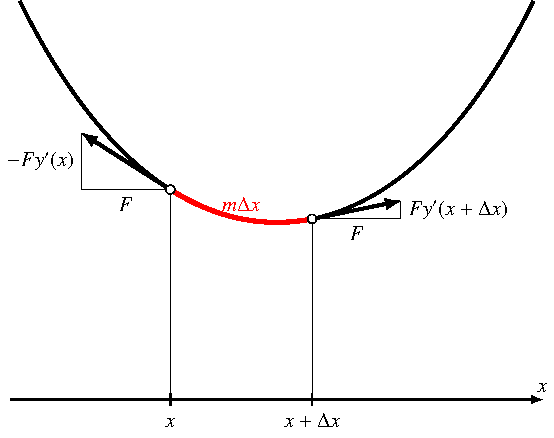
\includegraphics{chapters/50-ode/figures/kettenlinie.pdf}
\caption{Herleitung der Differentialgleichung der Kettenlinie
\label{numerik:kettenlinie}}
\end{figure}
Zunächst brauchen wir für eine Differentialgleichung, deren Lösung die
gesuchte Kurve beschreibt.
Zur Herleitung dient die Abbildung~\ref{numerik:kettenlinie}.
Die Masse des Seils zwischen den beiden Punkten $x$ und $x+\Delta x$
wird von den beiden eingezeichneten Kräften getragen.
Die horizontalen Komponenten tragen nicht dazu bei, das Seil zu
tragen, sie haben daher entlang des ganzen Seils immer die gleiche
Grösse $F$.
Die Masse des Seilstücks ist proportional zu seiner Länge,
der Proportionalitätsfaktor ist die lineare Massendichte $\mu$.
Nach dem dritten Newtonschen Gesetz
\index{Newton!drittes Gesetz von}
sind die vertikalen Kraftkomponenten gleich gross wie die Gewichtskraft
des Seilstücks:
\begin{align*}
F(y'(x+\Delta x)-y'(x))
&= \mu g\sqrt{(y(x+\Delta x)-y(x))^2+\Delta x^2}
\\
\intertext{oder nach Divison durch $F\Delta x$:}
\frac{y'(x+\Delta x)-y'(x)}{\Delta x}
&=\frac{\mu g}{F}\sqrt{1+\biggl(\frac{y(x+\Delta x)-y(x)}{\Delta x}\biggr)^2}.
\end{align*}
Schreibt man $a=\mu g/F$ und geht zur Grenze $\Delta x\to 0$ über,
erhält man die Differentialgleichung
\begin{equation}
y''(x)=a\sqrt{1+y'(x)^2}.
\label{numerik:kettenloesung}
\end{equation}
Diese Differentialgleichung hat die Funktion
\[
y(x) = \frac1a \cosh ax + C
\]
als Lösung, wie man durch Nachrechnen einsehen kann\footnote{
Man kann die Gleichung~\eqref{numerik:kettenloesung} natürlich auch direkt
lösen. Dazu bestimmt man zuerst die Funktion $z(x)=y'(x)$, welche die
Differentialgleichung
\[
z'(x)=a\sqrt{1+z(x)^2}
\]
erfüllt.
Diese Gleichung lässt sich durch Separation lösen:
\[
\begin{aligned}
\frac{dz}{dx}&=a\sqrt{1+z^2}
&&\Rightarrow&
\frac1a \int\frac{dz}{\sqrt{1+z^2}}&=\int \,dx
&&\Rightarrow&
\frac1a \asinh z &=x+C_1
&&\Rightarrow&
z(x)=\sinh a(x+C_1).
\end{aligned}
\]
Die Funktion $y(x)$ bekommt man jetzt durch Integration
\[
y(x)=\int z(x)\,dx = \frac1a \cosh a(x+C_1) + C_2,
\]
mit $C_1 = -x_0$ und $C_2=C$ genau die vorgeschlagene Lösung.
}.
Die Ableitungen von $y(x)$ sind
\begin{align*}
y' (x) &=  \sinh ax\\
y''(x) &= a\cosh ax.
\end{align*}
Eingesetzt in die Differentialgleichung erhält man
\begin{align*}
a\cosh ax&=a\sqrt{1+\sinh^2 ax},
\\
\intertext{was sich zu}
\cosh^2ax-\sinh^2ax&=1
\end{align*}
umformen lässt, diese Gleichung ist für hyperbolische Funktionen
immer erfüllt.

Die Differntialgleichung~\eqref{numerik:kettenloesung}
ist autonom, also sind auch verschobene Funktionen Lösungen.
Die allgemeine Lösung des Problems ist daher die Funktion
\begin{equation}
y(x)=\frac1a\cosh a(x-x_0) + C.
\label{numerik:ketteaC}
\end{equation}
Die Bedeutung der Konstante $C$ ist leichter verständlich, wenn man sie
als $C=y_0-1/a$ schreibt, also
\[
y(x)=\frac1a\cosh a(x-x_0) -\frac1a+y_0.
\]
Setzt man $x=x_0$ ein, findet man $y(x_0)=y_0$, d.~h.~der Punkt $(x_0,y_0)$
ist der Scheitelpunkt des Graphen von $y(x)$.

Damit kann jetzt das Anfangswertproblem gelöst werden.
Wir verlangen, dass die im Punkt $x=x_1$ der Funktionswert 
$y(x_1)=y_1$ sein soll, und die Steigung $y'(x_1)=m$.
Setzt man die Lösung~\eqref{numerik:ketteaC} in die Bedingung
für die Steigung ein, erhält man
\[
m=\sinh a(x_1-x_0)
\qquad\Rightarrow\qquad
\asinh m =a(x_1-x_0)
\qquad\Rightarrow\qquad
x_0=x_1-\frac1a\asinh m.
\]
Die Anfangsbedingung für $y(x_1)$ liefert
\begin{align*}
y_1
&=
y(x_1)
=
\frac1a\cosh a(x_1-x_0) + y_0 - \frac1a
=
\frac1a\cosh \asinh(m)+y_0-\frac1a
=
\frac1a\sqrt{1+m^2}+y_0-\frac1a
\\
\Rightarrow\quad
y_0
&= 
y_1+\frac1a-\frac1a\sqrt{1+m^2}.
\end{align*}
Damit ist das Anfangswertproblem vollständig gelöst, 
\begin{equation}
y(x)
=
\frac1a\cosh \bigl(a(x-x_1) + \asinh m\bigr)
+ y_1 - \frac1a\sqrt{1+m^2}
\end{equation}
ist die allgemeine Lösung zur Anfangsbedingung $y(x_1)=y_1$, $y'(x_1)=m$.

Mit dieser Lösung kann jetzt auch das Randwertproblem gelöst werden.
Es muss ein Wert $m$ gefunden werden, so dass $y(x_2)=y_2$,
man muss also die Gleichung
\[
y_2
=
\frac1a\cosh \bigl(a(x_2-x_1)+\asinh m\bigr) + y_1 - \frac1a\sqrt{1+m^2}
=:
f(m)
\]
nach $m$ auflösen.
Das ist leider nicht so einfach, weil $m$ in der transzendenten Funktion
$\asinh$ auftritt.

Wir können die Gleichung jedoch iterativ mit dem Newton-Verfahren
nach Satz~\ref{newton:satz} lösen.
Dazu brauchen wir die Ableitung von $f$, sie ist
\[
f'(m)
=
\frac{ \sinh (x_2-x_1+\asinh m) -m}{\sqrt{m^2+1}}.
\]
Damit können wir die Iterationsformel
\[
m_{\text{neu}} = m - \frac{f(m) - y_2}{f'(m)}
\]
für den korrekten Wert $m$ finden.
Sie kann leicht in Octave implementiert werden, wie Listing~\ref{numerik:ketteprog} zeigt.
%\lstinputlisting[style=Octave]{chapters/examples/kette.m}
%\begin{lstlisting}[style=Octave,caption={Octave-Programm zur Bestimmung der Anfangssteigung $m$ im Kettenlinien-Problem}]
%\begin{lstlisting}[style=Octave, caption={Octave-Programm}, captionpos={b}, label={numerik:ketteprog}]
%\verbatiminput{chapters/examples/kette.m}

In Tabelle~\ref{numerik:kette-newton} ist der Gang der Berechnung
für den Fall $x_1=-1$, $x_2=2$, $y_1=1$ und $y_2=2$  mit dem
Startwert $m=0$ dargestellt.
Wie erwartet ist die Konvergenz quadratisch, in jedem Schritt verdoppelt
sich die Anzahl korrekter Stellen.
In Abbildung~\ref{numerik:kette-newton-graph} sind die Graphen von $y(x)$
zu den im Newton-Algorithmus ermittelten Werten von $m=y'(x_1)$ blau
dargestellt, die Lösungskurve ist rot.
\begin{table}
\centering
\begin{tabular}{|r|>{$}c<{$}|>{$}c<{$}|}
\hline
  &                      m                 &           f(m)               \\
\hline
 1&\phantom{-}           0.0000000000000000& \phantom{-}8.0676619957777653\\
 2&         -            0.8053266839760436& \phantom{-}2.5748454835378896\\
 3&         -\underline{1}.3999183852140562& \phantom{-}0.5757860863682827\\
 4&         -\underline{1.6}180720459804230& \phantom{-}0.0383682292517731\\
 5&         -\underline{1.634}7219547661627& \phantom{-}0.0001812733120350\\
 6&         -\underline{1.63480136}59846743& \phantom{-}0.0000000040625958\\
 7&         -\underline{1.634801367764473}7& \phantom{-}0.0000000000000004\\
 8&         -\underline{1.6348013677644739}&           -0.0000000000000002\\
\hline
\end{tabular}
\caption{Numerische Lösung des Randwertproblems für die Kettenlinie
mit Randbedingungen $x_1=-1$, $x_2=2$, $y(x_1)=y_1$ und $y(x_2)=y_2$.
\label{numerik:kette-newton}}
\end{table}
\begin{figure}
\centering
%\includegraphics[width=\hsize]{chapters/images/numerik-6.pdf}
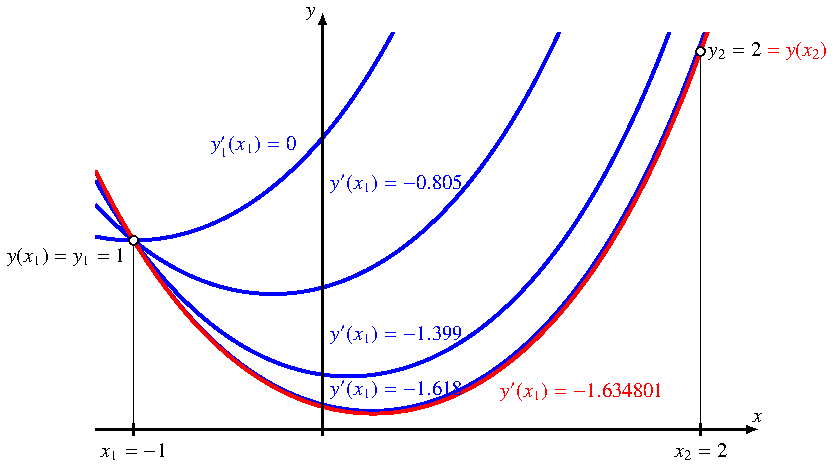
\includegraphics{chapters/50-ode/figures/kettenloesung.pdf}
\caption{Iterative Bestimmung der Kettenlinie zwischen
den Punkten $(-1,2)$ und $(2,2)$ mit Hilfe des Newton-Algorithmus.
\label{numerik:kette-newton-graph}}
\end{figure}
\end{loesung}
\begin{lstlisting}[style=Octave,caption={Octave-Programm zur Bestimmung der Anfangssteigung $m$ im Kettenlinien-Problem}, captionpos={t}, label={numerik:ketteprog}]
global x1 = -1
global x2 =  2
global y1 =  1
global y2 =  2

function v = f(m)
        global x1 x2 y1 y2
        v = cosh(x2 - x1 + asinh(m)) + y1 - y2 - sqrt(1 + m^2);
endfunction

function v = fprime(m)
        global x1 x2 y1 y2
        v = (sinh(x2 - x1 + asinh(m)) - m)/sqrt(1 + m^2);
endfunction

m = 0;

for i = (1:10)
        printf("%2d   %20.16f %20.16f\n", i, m, f(m));
        m = m - f(m)/fprime(m);
endfor
\end{lstlisting}

\subsection{Schiess-Verfahren\label{numerik:schiess-verfahren}}
\index{Schiess-Verfahren}%
Wenn man experimentell versucht, ein Ziel zu treffen, dann wird man
in wiederholten Versuchen die Richtung anpassen, so dass man dem Ziel
immer näher kommt.
Genau dies haben wir in der Aufgabe~\ref{numerik:aufgabe-seil} gemacht,
wo wir iterativ die noch unbekannen Anfangsbedingung $y(x_1)=m$ bestimmt
haben, mit der die Lösung durch den rechten Randpunkt $y(x_2)=y_2$ geht.

Auch in der Aufgaben~\ref{numerik:aufgabe-ball} konnten wir die
Parameter direkt bestimmen.
Doch auch dort läuft die Lösung auf die Bestimmung einer 
geeigneten Anfangsbedingung hinaus.
Der $y$-Wert zur Zeit $p/v_x$ hängt von der Vertikalgeschwindigkeit ab,
wir bezeichnen ihn mit $h(v_y)$.
Man verändert also $v_y$, bis die Gleichung $h(v_y)=0$ erfüllt ist.
Um das Randwertproblem zu lösen, muss man also die Gleichung $h(v_y)=0$
numerisch lösen.

Man kann dies z.~B.~dadurch machen, dass man nach zwei Werten von $v_y$
sucht, so dass die zum einen gehörige Bahn unter dem Punkt $P$ durchgeht,
während der Ball im anderen Fall darüber hinwegfliegt.
Durch wiederholte Halbierung des Intervalls kann man dann den korrekten
Wert für $v_y$ immer genauer eingrenzen%
\footnote{%
Tatsächlich wird dieses Verfahren in der Artillerie verwendet.
\index{Artillerie}%
Der Schiesskommandant beobachtet die einschlagenden Granaten und kommandiert
Änderungen der Anfangs-Elevation an die Geschützbatterien.
Dabei sucht er Einschläge, die aus seiner Perspektive vor bzw.~hinter
dem Ziel liegen, und halbiert dann das Intervall, bis die Einschläge dem
Ziel genügend nahe kommen.}.
Der Nachteil dieses Verfahrens ist, dass mit jedem Schritt die Genauigkeit
nur um in Bit ansteigt, es sind also sehr viele Iterationen notwendig.

Schnellere Konvergenz kann mit dem Newton-Verfahren erreicht werden,
welches in Anhang~\ref{chapter:newton} beschrieben wird.
\index{Newton-Verfahren}%
Für die Anwendung des Newton-Verfahrens auf das Randwert-Problem
ist die Bestimmung der Steigung der Funktion nötig, die die Abweichung
der Kurve von der Randbedingung am rechten Rand angibt.
Wir müssen also berechnen, wie schnell sich $y(p/v_x)$ ändert,
wenn $v_y$ verändert wird.
Dies ist die Ableitung
\[
h'(v_y)= \frac{\partial y}{\partial v_y},
\]
ein Eintrag der Jacobi-Matrix.
In Abschnitt~\ref{grundlagen:jacobi} wurde gezeigt, wie man auch für
die Jacobi-Matrix eine Differentialgleichung aufstellen kann, die
man natürlich ebenfalls mit den früher beschriebenen numerischen
Bibliotheken lösen kann.

Das Randwertproblem kann daher mit folgendem Algorithmus numerisch gelöst
werden.
\begin{enumerate}
\item Beginne mit einer Schätzung für $v_y$
\item Finde numerisch die Lösung des Anfangswertproblems mit $v_y$
als anfängliche Vertikalgeschwindigkeit.
Berechnet dabei auch die Jacobi-Matrix
\item Lese die $h(v_y)$ aus der Lösung zur Zeit $p/v_x$ ab, und $h'(v_y)$
aus der Jacobi-Matrix und verwendet den Newton-Algorithmus
(Satz~\ref{newton:satz}), um eine verbesserte Schätzung von $v_y$ 
zu bekommen.
\item Wiederhole Schritte 2 und 3 bis die Randbedingung für $t=p/v_x$
genügend genau erfüllt ist.
\item Die Lösung des Anfangswertproblems mit diesem $v_y$ ist die
Lösung des gestellten Randwertproblems.
\end{enumerate}

\begin{beispiel}
\begin{figure}
\centering
%\includegraphics{chapters/images/randwert-1.pdf}
\caption{Lösungen des Anfangswertproblems~\eqref{numerik:ball-dgl-1} und
\eqref{numerik:ball-dgl-2}.
Das Newton-Verfahren korrigiert $v_y$ derart, dass $h(v_y)=0$ wird.
So wird die Lösung des Randwertproblems (rot) gefunden.
\label{numerik:randwert-bild}}
\end{figure}
Wir führen den eben skizzierten Algorithmus für das Ball-Problem durch.
Um die Jacobi-Matrix zu berechnen, müssen wir die Ableitung von $f$ berechnen:
\begin{equation}
\frac{\partial f(x,y)}{\partial y}
=
\begin{pmatrix}
0& 0& 1& 0\\
0& 0& 0& 1\\
0& 0& 0& 0\\
0& 0& 0& 0
\end{pmatrix}.
\end{equation}
Da die rechte Seite nicht von $y$ abhängt, können wir die Gleichung für
die Jacobi-Matrix ganz unabhängig von $y$ lösen.
Da $F$ so einfach ist, kann man das Matrizenprodukt direkt ausrechnen, 
so wird die Differentialgleichung für $J$
\begin{equation}
\begin{pmatrix}
J'_{11}&J'_{12}&J'_{13}&J'_{14}\\
J'_{21}&J'_{22}&J'_{23}&J'_{24}\\
J'_{31}&J'_{32}&J'_{33}&J'_{34}\\
J'_{41}&J'_{42}&J'_{43}&J'_{44}
\end{pmatrix}
=
\begin{pmatrix}
0& 0& 1& 0\\
0& 0& 0& 1\\
0& 0& 0& 0\\
0& 0& 0& 0
\end{pmatrix}
\begin{pmatrix}
J_{11}&J_{12}&J_{13}&J_{14}\\
J_{21}&J_{22}&J_{23}&J_{24}\\
J_{31}&J_{32}&J_{33}&J_{34}\\
J_{41}&J_{42}&J_{43}&J_{44}
\end{pmatrix}
=
\begin{pmatrix}
J_{31}&J_{32}&J_{33}&J_{34}\\
J_{41}&J_{42}&J_{43}&J_{44}\\
     0&     0&     0&     0\\
     0&     0&     0&     0
\end{pmatrix}.
\end{equation}
\begin{table}
\centering
\begin{tabular}{|>{$}r<{$}|>{$}r<{$}|>{$}r<{$}|>{$}r<{$}|>{$}r<{$}|>{$}r<{$}|>{$}r<{$}|>{$}r<{$}|}
\hline
n&    v_y&    t& x(t)&      y(x)&\displaystyle\frac{\partial^{\mathstrut}y}{\partial v_y}&v_{y,\text{new}}&\Delta\\
\hline
0& 7.0000&  2.5& 20.0&-13.156250&  2.5& 12.26250000& -5.2625000000\\
1&12.2625&  2.5& 20.0& -0.000004&  2.5& 12.26250145& -0.0000014458\\
2&12.2625&  2.5& 20.0&  0.000000&  2.5& 12.26250143&  0.0000000204\\
\hline
\end{tabular}
\caption{Newton-Algorithmus für das Ball-Problem, Resultate der numerischen
Rechnung.
$v_y$ wird in drei Schritten mit einer Genauigkeit von mehr als 10 Stellen
gefunden.
\label{numerik:newton-resultate}}
\end{table}%
Daraus kann man ablesen, dass die Elemente $J_{3j}$ und $J_{4j}$ sich
nicht ändern, sie bleiben also konstant.
Aber auch in den ersten zwei Zeilen können sich nur die Elemente $J_{13}$
und $J_{24}$ ändern, die Differentialgleichungen für diese Elemente
sind
\begin{align*}
J'_{13}&=1\\
J'_{24}&=1
\end{align*}
oder in Matrixform:
\begin{equation}
J(x) = \begin{pmatrix}
1&0&x&0\\
0&1&0&x\\
0&0&1&0\\
0&0&0&1
\end{pmatrix}.
\end{equation}
Die Lösung $J_{13}(x)=x$ und $J_{24}=x$.
Damit haben wir die nötige Information, um den Newton-Algorithmus
durchzuführen.
In Tabelle~\ref{numerik:newton-resultate}
sind die Resultate der numerischen Rechnung zusammengestellt.
Es zeigt sich, dass der korrekte Wert für $v_y$ in drei Iterationen
mit 10 Stellen Genauigkeit gefunden werden kann.
Damit ist das Randwertproblem numerisch gelöst.
\end{beispiel}


\section*{Übungsaufgaben}
\rhead{Übungsaufgaben}
\aufgabetoplevel{chapters/50-ode/uebungsaufgaben}
\begin{uebungsaufgaben}
\uebungsaufgabe{5001}
\uebungsaufgabe{5002}
\end{uebungsaufgaben}

